\documentclass[12pt]{article}
\usepackage[margin=1in]{geometry}
\usepackage{hyperref}
\usepackage{color}

\hypersetup{
    colorlinks,
    citecolor=black,
    filecolor=black,
    linkcolor=black,
    urlcolor=black
}

\title{RISC-V: A Didactic Platform \\
\large Documentation}

\author{Jules PERRIN, Professor: Theo Kluter}
\date{\today}

\begin{document}
\maketitle
\tableofcontents

\section{Introduction}
This document describes the RV32IM processor and its architecture. I've tried to make it as clear 
as possible such that everyone with a basic knowledge of computer architecture can understand it.
It will describe each significant module of the processor, what it does and what are the different
inputs and outputs with an image of the module.
It is recommended to follow this document with the source code of the processor, which is available
in the Verilog folder of the project.
Don't hesitate to use the table of contents to navigate through the different parts of the document.
If you see any mistake or are confused by something don't hesitate to contact me at the mail address
\href{mailto:jules.perrin@epfl.ch}{jules.perrin@epfl.ch}.

\section{Fetch}
\subsection{IF Stage}

\begin{figure}[H]
\centering
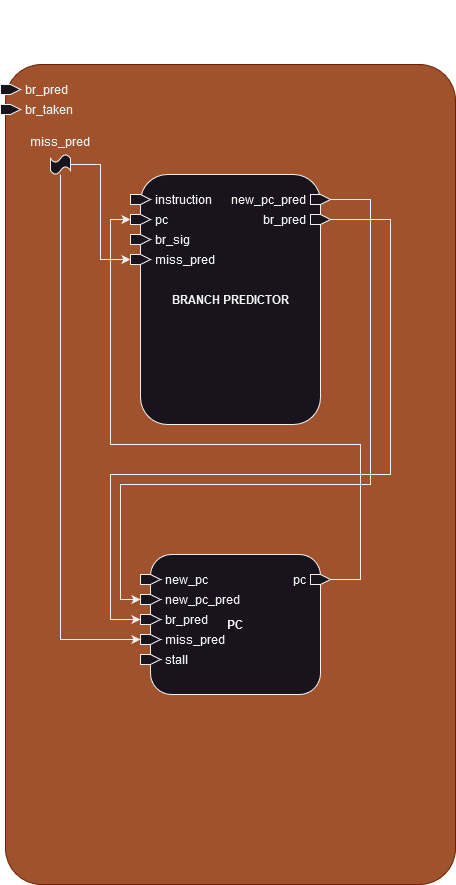
\includegraphics[width=0.5\textwidth]{../diagrams/fetch/if_stage.png}
\caption{Diagram of the IF Stage}
\label{fig:IF_Stage}
\end{figure}

The IF stage is responsible for fetching the next instruction from the ROM and passing it to the ID stage. 
The IF stage contains two different modules: the PC and the branch predictor.
The IF stage is the only stage that computes a value outside of a value, it uses the $br\_pred$ signal and the 
$br\_taken$ signal to compute if there is a miss prediction such that the PC and the branch predictor can be updated
accordingly. \\

Signals:
\begin{enumerate}
    \item Input: $br\_pred$, This signal is representing the state of the prediction made by the branch predictor in the EX stage.
    \item Input: $br\_taken$, This signal is representing the state of the branch in the EX stage.
    \item Output: $miss\_pred$, This signal is representing if there is a miss prediction or not.
\end{enumerate}



\end{document}
